\documentclass[twoside]{article}
\input{ISC18-english.sty}
%%%%%%%%%%%%%%%%%%%%%%%%%%%%  Make sure to compile twice for proper cross-references. %%%%%%%%%%%%%%%%%%%%%%%
%%%%%%% For proper display of references, compile the document twice. %%%%%%%%%%%%%%%%%%%%% 
%%%%%%%%%%%%%%% If using TeX Live, compile using pdflatex command %%%%%%%%%%%%%%%%%%%%%%%
\begin{document}
\thispagestyle{empty}
%%%%%%%%%%%%%%%%% Article title header  %%%%%%%%%%%%%%%%%%%%
\fancyhead[LE]{Short Article Title}
%%%%%%%%%%%%%%%%% Article authors header   %%%%%%%%%%%%%%%%%%%%
\fancyhead[RO]{Short Authors' Names}
\begin{center}
{
\includegraphics [height=25mm, width=150.3mm] {Images/isc18E}} \\
\vspace*{-1.8cm}
%\begin{center}
%\color{blue} 
%{\hspace{0.1cm}\rule{\textwidth}{1mm}}\\
%\end{center}
\vspace*{4cm}
%%%%%%%%%%%%%%%%% Article title  %%%%%%%%%%%%%%%%%%%%
{\Large \bf  Maximum likelihood estimation of length-biased censored data under Frank copula dependency}\\
%%%%%%%%%%%%%%%%% Article authors and affiliations %%%%%%%%%%%%%%%%%%%%
%{\bf
 %Motahareh Barazesh\footnote[1]{{\bf Corresponding Author:} {\tt m.barazesh@math.uk.ac. }} , Ayyub Sheikhi \\
%Department of Statistics, Faculty of Mathematics and Computer,\\
%Shahid Bahonar University of Kerman, Kerman, Iran}
\end{center}
\rule{\textwidth}{0.2mm}\\
%%%%%%%%%%%%%%%%% Article abstract  %%%%%%%%%%%%%%%%%%%%
\noindent{\bf Abstract:}\\
Ignoring censoring causes bias in survival analysis, especially for length-biased data. In this work, we estimate parameters in length-biased survival data with dependent censoring using a copula function to model the dependency between survival and censoring times. Extensive simulations show that our approach improves estimation accuracy and simplifies computing conditional probabilities of copulas. A real-data application is also provided.\\ 
\noindent{\bf Keywords:} 
Survival analysis, Length-biased, Copula, Parameter estimation \\
\noindent{\bf Mathematics Subject Classification (2010):} $\rm 62H05$, $\rm 62Hxx$, $\rm 62N02 $. \\
\hspace{1cm}\rule{\textwidth}{0.2mm}\\
%%%%%%%%%%%%%%
\section{Introduction}
Survival analysis is the analysis of time-to-event data such as the length of time from a
time origin to an endpoint of interest. Such analytical methods are usually used to analyze
data collected prospectively in time, such as data from a prospective cohort study or data
collected for a clinical trial \cite{kartsonaki2016survival}.\\ One of the main statistical challenges in survival analysis is handling censored data.
This issue occurs when we have some information about individual survival time, but in
some cases, we do not know the survival time exactly \cite{singh2011survival}

The main aim of survival analysis is focus to the time between an initiating event and a specific or terminating event, such as the time from the onset of a
disease to relapse or death due to the disease, however, sometimes the onset is not clearly
specified \cite{akbari2025pseudo}. In recent years, copula function was applied in survival analysis, especially on length
biased. For some instances,  \cite{rabhi2020nonparametric} have used copulas for
modeling dependence when the collected data are length-biased and account for both
informative censoring.\\
The main aim of this paper is introduce statistical method for analyzing length biased data subject to dependent censoring. We express parametric likelihood method by
assuming a copula between residual life and residual censoring time and assuming that  left truncation time is independent of residual life and censoring time. 
\section{Distribution of length-biased survival data} 
Inspiring the the seminal work of  \cite{sklar1959fonctions}, for two random variables $X$ and $Y$, there exists  a function $C: \left[0,1 \right]^2 \rightarrow \left[0,1 \right] $
such that
\begin{equation}
\label{eq:1-4}
F_{X,Y}(x,y)=C(F_X(x),F_Y(y)),
\end{equation}
where $F_{X,Y}: \mathbb{R}^2 \rightarrow \left[0,1 \right] $
is the joint distribution function of  the random vector $({X,Y})$ and $F_X,\; F_Y: \mathbb{R} \rightarrow \left[0,1 \right]$ are distribution functions of random variables $X$ and $Y$, respectively.  The function $C: \left[0,1 \right]^2 \rightarrow \left[0,1 \right] $ is a copula if and only if it is a  grounded, uniformly marginal and $2-$increasing bivariate function. Hence their joint density copula, if exists, is just function $c(.,.)$ such that
\begin{equation}
\label{eq:1-5}
f_{X,Y}(x,y)=f_X(x)f_Y(y)c(F_X(x),F_Y(y)).
\end{equation}
Let $\tilde{T}$ be survival time in the unbiased population with probability density function $\tilde{f}(t)$, cumulative distribution $\tilde{F}(t)$, and survival function $\tilde{S}(t)=1-\tilde{F}(t)$.
Suppose a random sampling time occurs uniformly over the calendar time axis.
Let $A$ denote the observed \emph{ truncation time} and $V$ is
the residual life  and $C$ is the residual censoring time after sampling.
So, $T=A+V$ is the total survival time and $U=A+C$ is the total censoring time.
In a random sample of $n$ independent subjects, the length biased data in the absence of covariates consist of $(y_i,A_i,{\delta_i})$ 
where $y_i=A_i+\min(V,C)$  and ${\delta_i}=I(V_i\leqslant C_i)$ is censoring indicator.
This case  is referred to as length-biased sampling. Biased sampling occurs when an investigator naturally collects samples from a population, but the sampling distribution is different from the target population. It happens because not every unit in the population has an equal chance to be sampled when the natural sampling plan is adopted \cite{qin2017biased}. Because individuals with longer lifetimes are more likely to be present at the
sampling time, the observed distribution of $T$ is known as length-biased.  That is,
$$  f_T^{\text{(obs)}}(t)
  = \frac{t\,\tilde{f}(t)}{\mu}, \qquad
  \mu = E[\tilde{T}] = \int_0^\infty t\,\tilde{f}(t)\,dt,
  \quad t>0.$$
  This is the standard form of the length-biased density and the conditional density of $A$ given $T=t$ can be readily obtained as
$  f_{A\mid T}(a\mid t) = \frac{1}{t}, \qquad 0<a<t,$
which means the sampling time is equally likely to fall anywhere in the interval $(0,t)$. Also,  by the aid of multiplication rule, their joint density is obtained as
$$  f_{(A,T)}(a,t) = \frac{\tilde{f}(t)}{\mu}, \qquad t>a>0,$$
 Integrating over $t$ of this density helps us to acquire  the marginal density of $A$ as 
$  f_A(a)  = \frac{\tilde{S}(a)}{\mu},  \\ a>0.$ 
Similarly, since $V=T-A$, the same expression holds for $f_V(v)$ can be represented as
$f_V(v) = \frac{\tilde{S}(v)}{\mu}, \qquad v>0.$
Thus we have
$$ f_A(t\mid X) = f_V(t\mid X)
  = \frac{\tilde{S}(t\mid X)}{\mu(X)}, \qquad t>0,$$ 
  
  We use these densities to explore the parameter estimation in length-biased censored survival data using a copula-based approach. For this, we follow 
  \cite{emura2018analysis} and consider a bivariate survival function  
\begin{equation}\label{abc}
P(V>v,C>c)=C_{\theta}(S_V(v) , S_C(c)),
\end{equation}
where $S_V(v)=P(V>v), \ \ S_C(c)=P(C>c)$ are respectively the marginal survival function of $V$ and $C$, and $ C_{\theta}$ is a copula with parameter ${\theta}$.
According to \eqref{abc}  and using facts $T=A+V$ and $ U= A+C$, via some algebra we obtain the joint survival of $T$ and $U$ using the copula of $V$ and $C$ as
\begin{equation}
P(T>t,U>t) =\int C_{\theta}(S_V(t-a) , S_C(t-a))f_A(a) d(a). 
\end{equation}
We apply these relations to carry out a parameter estimation.
For $n$ independent cases and  their corresponding observed values  $(y_i,A_i,\delta_i), i=1,2,...,n$,  the likelihood function is constructed. The  likelihood can be used to estimate parameters of the length-biased model. 

The following proposition explores our results under the exponential marginals and Frank copula.
 \begin{pro}
\label{ex1}
Let  marginal  distributions of  random variables  $V$  and $C$ follow exponential  as $S_V(v, \lambda_1)=e^{-\lambda_1 v}$  and $S_C(c, \lambda_2)=e^{-\lambda_2 c}$ where $\lambda_1>0$ and $\lambda_2>0$ are their parameters respectively. Also assume that they are connected via the Frank copula. Then  log-likelihood  function for observed  values $(y_i,A_i,\delta_i), i=1,2,...,n$,  is 
Defined as follows:

$$
\begin{aligned}
\ell = \sum_{i=1}^{n} \delta_i &\log \int \frac{
\lambda_1 S_1^{(i)} e^{-\theta S_1^{(i)}} 
\left( e^{-\theta S_2^{(i)}} - 1 \right)
}{
(e^{-\theta} - 1) + 
\left( e^{-\theta S_1^{(i)}} - 1 \right)
\left( e^{-\theta S_2^{(i)}} - 1 \right)
} \, f_A(a_i) \, da_i \\
&\quad + (1 - \delta_i) \log \int \frac{
\lambda_2 S_2^{(i)} e^{-\theta S_2^{(i)}} 
\left( e^{-\theta S_1^{(i)}} - 1 \right)
}{
(e^{-\theta} - 1) + 
\left( e^{-\theta S_1^{(i)}} - 1 \right)
\left( e^{-\theta S_2^{(i)}} - 1 \right)
} \, f_A(a_i) \, da_i,
\end{aligned}
$$
 where  $S_j^{(i)} = e^{-\lambda_j (y_i - a_i)}, \ \ j = 1, 2$ are the corresponding  survival functions.

 \end{pro}
\section{Numerical Analysis}
%%%%%%%%%%%%%%%%%%%%%%%%%%%%%%% Unnumbered formula %%%%%%%%%%%%%%%%%%%%%%%
In this section we provide the numerical studies, including simulated analysis and real data application.
\subsection{Simulation Study}
In order to explain and  assess our approach,  in this section  we used the Mont-Carlo method in our simulation study. We  considered exponential marginals and Frank copula.
In this scenario, we supposed that residual life  $V$ and residual censoring $C$ follow exponential distributions with parameters $\lambda_1$ and $\lambda_2$ respectively and truncation time A has uniform distribution on $(0.1,10.1)$. We also assume that their dependency is modeled by the Frank copula with parameter $\theta$. Assuming $\lambda_1=1.2$ and $\lambda_2=1.5$, we considered two scenarios for the dependency structure, one whit a positive  relationship and one whit negative relationship; which we assumed  $\theta=5.5$ for relationship. We generated 1000 samples and by constructing  the objective function \eqref{abc} we estimated  parameters. In order to estimate a stable and robust estimator, we repeated $M=50, 100$ and $200$ times our parameter estimation.
\begin{table}[h]
\begin{center}
\renewcommand{\arraystretch}{0.7}
\small
\begin{tabular}{|c|ccc|ccc|ccc|}
\hline
\multicolumn{10}{|c|}{Repetition} \\
\hline
 & \multicolumn{3}{c|}{$M=50$} & \multicolumn{3}{c|}{$M=100$} & \multicolumn{3}{c|}{$M=200$} \\
\hline
Parameter & $\theta$ & $\lambda_1$ & $\lambda_2$ & $\theta$ & $\lambda_1$ & $\lambda_2$ & $\theta$ & $\lambda_1$ & $\lambda_2$ \\
\hline
Estimate & 5.492 & 1.200 & 1.499 & 5.503 & 1.211 & 1.514 & 5.505 & 1.206 & 1.505 \\
Bias & -0.007 & 0.0002 & -0.0006 & 0.003 & 0.011 & 0.014 & 0.005 & 0.006 & 0.005 \\
MSE & 0.014 & 0.007 & 0.012 & 0.007 & 0.005 & 0.007 & 0.009 & 0.006 & 0.008 \\
\hline
\end{tabular}
\end{center}
\caption{The estimated values of parameters and their biases and MSE.}
\label{tab2}
\end{table}
Under the assumption of $\theta=5.5$, Table \ref{tab2} provides the mean of our estimated parameters as well as their bias and mean square error (MSE)  for $ M=50, 100, 200$, see also  Figure \ref{fig1}.
\newpage
\begin{figure}[th]
\begin{center}
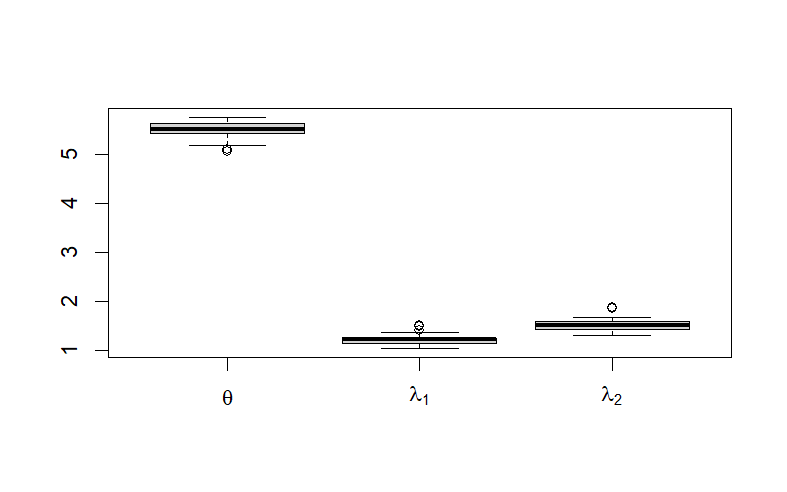
\includegraphics[width=7cm,height=6cm]{Images/figexp in lb.png}
\vspace{-1.5cm}
\caption{\footnotesize{Convergence of the parameter estimation  in  length-biased simulated data with Frank copula and exponential marginals.}}\label{fig1}
\end{center}
\end{figure}
\subsection{Real Data}
To demonstrate the proposed method, we applied it to  real data namely, Rotterdam data set, which is   available in the \texttt{survival} package in R.
This data set is a classic resource for studying breast cancer prognosis under left truncation and right censoring, and we used it to illustrate our approach. The data set has 2982 primary breast cancer patients treated at the Rotterdam Tumor Bank. We considered ``rtime" as the survival time, ``death" as censoring indicator and  ``year" as the left truncation time.
For fitting marginal distributions   of survival time ($V$) and censoring time ($C$), we chose four competitive distributions:  Exponential, Weibull, Gamma and Lognormal.   Based on the results of the top panel of Table \ref{tab:cop}, we realized that both survival and censoring times follow Weibull distributions. So, we proceed with  parmeter estimation by optimizing the log likliehood  function by considering the Weibull  distribution as the marginal.  To model their dependency, in this optimization process we considered three copulas:  Frank, Joe   and Ali Mikhail Haq (AMH). The results are represented in the  Table \ref{tab:cop}.
\begin{table}[h]
\begin{center}
\renewcommand{\arraystretch}{0.7}
\setlength{\tabcolsep}{3pt}
\small
\begin{tabular}{|l|l|c|c|c|c|c|c|c|c|}
\hline
\multicolumn{10}{|c|}{Results for the Rotterdam data set} \\
\hline
\multicolumn{2}{|c|}{} & \multicolumn{5}{c|}{Parameter estimates} & \multicolumn{3}{c|}{Criteria} \\
\hline
Data set & Copula & $\hat{\alpha}_1$ & $\hat{\alpha}_2$ & $\hat{\lambda}_1$ & $\hat{\lambda}_2$ & $\hat{\theta}$ & LL & AIC & BIC \\
\hline
Rotterdam & Frank   & \textbf{1.04} & \textbf{1.093} & \textbf{25.5} & \textbf{18.20} & \textbf{-20.35} & \textbf{20425.59} & \textbf{40865.18} & \textbf{40899.54} \\
~ & Joe     & 1.03  & 1.089  & 27.18 & 19.033 & 1.588 & 145916.5 & 291847.1 & 291881.3 \\
~ & AMH     & 1.039 & 1.089  & 26.95 & 18.998 & -0.982 & 21067.53 & 42149.06 & 42183.42 \\
\hline
\end{tabular}
\end{center}
\caption{The ML estimated values of parameters and criteria for assuming different joint distributions for Rotterdam data set.}
\label{tab:cop}
\end{table}
\section*{Discussion and Conclusions}   
We modeled the dependency of survival time and censoring time in length-biased data using a copula function. While we assumed truncation time is independent of residual time and censoring, this can be extended. Future work may consider the case where  truncation time depends on residual time, residual censoring, or both.
\begin{thebibliography}{9}
\bibitem[Kartsonaki (2016)]{kartsonaki2016survival}
Kartsonaki C. (2016), Survival analysis, {\it Diagnostic Histopathology} 22, 7, 263--270.

\bibitem[Singh and Mukhopadhyay (2011)]{singh2011survival}
Singh R. and Mukhopadhyay K. (2011), Survival analysis in clinical trials: Basics and must know areas, {\it Perspectives in Clinical Research} 2, 4, 145--148.

\bibitem[Kaplan and Meier (1958)]{kaplan1958nonparametric}
Kaplan E.L. and Meier P. (1958), Nonparametric estimation from incomplete observations, {\it Journal of the American Statistical Association} 53, 282, 457--481.

\bibitem[Zheng and Klein (1995)]{zheng1995estimates}
Zheng M. and Klein J.P. (1995), Estimates of marginal survival for dependent competing risks based on an assumed copula, {\it Biometrika} 82, 1, 127--138.

\bibitem[Shih and Louis (1995)]{shih1995inferences}
Shih J.H. and Louis T.A. (1995), Inferences on the association parameter in copula models for bivariate survival data, {\it Biometrics} 51, 1384--1399.

\bibitem[Akbari et al. (2025)]{akbari2025pseudo}
Akbari M., Rad N.N. and Chen D.G. (2025), Pseudo-Observation Approach for Length-Biased Cox Proportional Hazards Model, {\it Biometrical Journal} 67, 6, e70094.

\bibitem[Nowell et al. (1988)]{nowell1988length}
Nowell C., Evans M.A. and McDonald L. (1988), Length-biased sampling in contingent valuation studies, {\it Land Economics} 64, 4, 367--371.
   
 \bibitem[Keiding (1991)]{keiding1991age}
Keiding N. (1991), Age-specific incidence and prevalence: a statistical perspective, {\it Journal of the Royal Statistical Society Series A: Statistics in Society} 154, 3, 371--396.
   
\bibitem[Cox (2005)]{cox2005some}
Cox D. (2005), Some sampling problems in technology, {\it Selected Statistical Papers of Sir David Cox} 1, 81--92.
   
 \bibitem[Rabhi and Bouezmarni (2020)]{rabhi2020nonparametric}
Rabhi Y. and Bouezmarni T. (2020), Nonparametric inference for copulas and measures of dependence under length-biased sampling and informative censoring, {\it Journal of the American Statistical Association} 115, 531, 1268--1278.  
   
\bibitem[Durante and Sempi (2015)]{durante2015principles}
Durante F. and Sempi C. (2015), {\it Principles of copula theory}, CRC Press.

\bibitem[Qin (2017)]{qin2017biased}
Qin J. (2017), {\it Biased sampling, over-identified parameter problems and beyond}, Springer.
\bibitem[Sklar (1959)]{sklar1959fonctions}
Sklar A. (1959), Fonctions de r\'epartition \`a n dimensions et leurs marges, {\it Annales de l'ISUP} 8, 3, 229--231.

\bibitem[Emura and Chen (2018)]{emura2018analysis}
Emura T. and Chen Y.H. (2018), {\it Analysis of survival data with dependent censoring: copula-based approaches}, Springer.
\end{thebibliography}
 \end{document}

